\section{Speed Measurements} \label{sec:measurements-speed}
In this chapter the generated data with CPlan \ref{CPlan} is compared and analysed.

\begin{figure}
    \centering
    \begin{mdframed}[style=mdthight]
        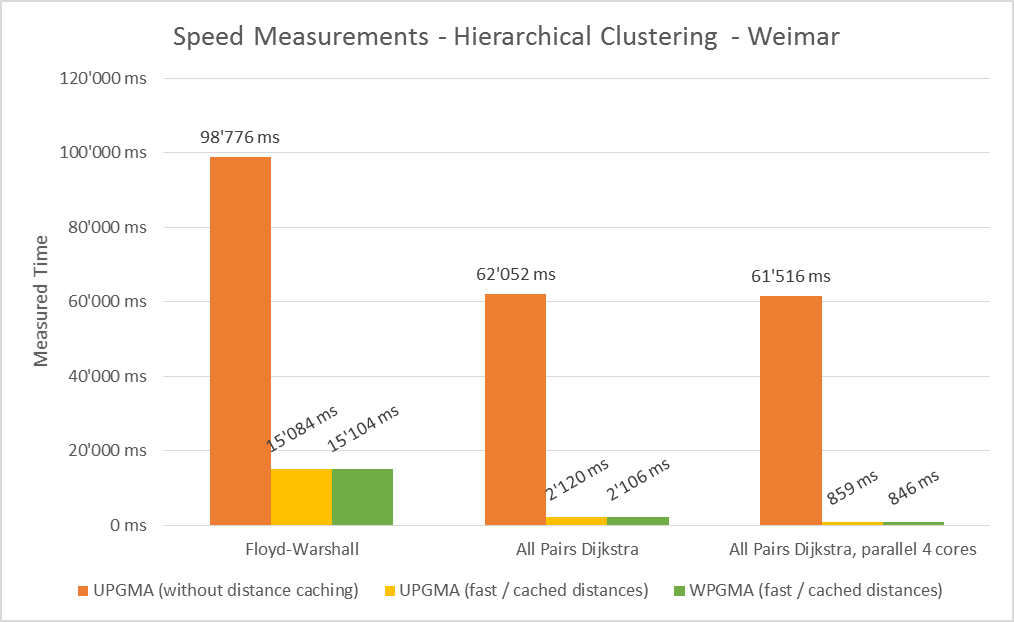
\includegraphics[width=\textwidth]{hierarchical_clustering_speed.png}
    \end{mdframed}
    \caption{\label{fig:hierarchical_clustering_speed}}
\end{figure}

\begin{figure}
    \centering
    \begin{mdframed}[style=mdthight]
        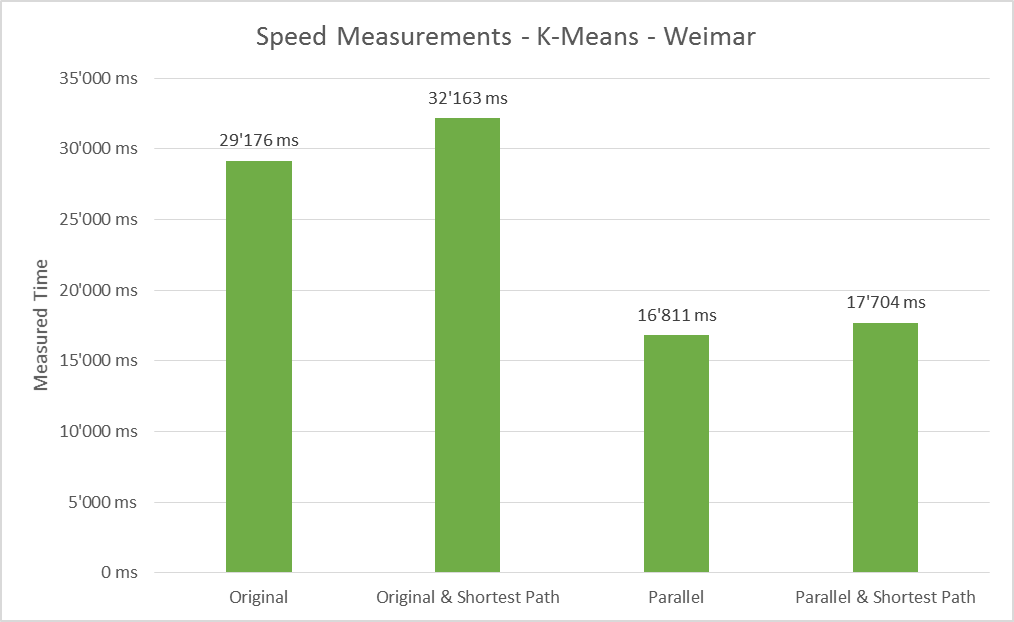
\includegraphics[width=\textwidth]{kmeans_speed.png}
    \end{mdframed}
    \caption{\label{fig:kmeans_speed}}
\end{figure}

TODO: Description of speed measurements here. 

TODO: Table of speed measurements here.

\section{Cluster Analysis}
\label{sec:measurements-cluster-analysis}
In this chapter the provided measurement methods \ref{sec:clusterRating} are used to compare different districts/areas. The following images were generated with the cluster algorithm FastUPGMA \ref{sec:UPGMAandWPGMA} on Weimar with \textit{Modified Output} and \textit{Number of Clusters} count 16.

\subsection{Measured Data}
\label{sec:ClusterAnalysisMeasurements}
The following table \ref{tab:cluterAnalysisDescription} contains the parameters with additional descriptions. Extended information can be found below the table. Of every parameter the minimal (min), maximal (max), mean (average) and the median value can be calculated.

\begin{table}[h]
\begin{center}
    \begin{tabular}{ | l | l |} \hline 
        \textbf{Parameter} & \textbf{Description} \\
        \hline
        Total Area &  Area of the convex hull \\ \hline
        Total Length & Sum of the street length \\ \hline
        Density & 'Total Area' divided by 'Total Length'  \\ \hline
        
        Street Length Min/Max/Mean & Shortest/Longest/Average street length  \\ \hline
        Street Length Median & Middle value of the length dataset \\ \hline
        Street Length Variance & Sigma of the normal distribution curve of the variance \\ \hline
        
        Vertex Connections & Mean connected edges per vertex  \\ \hline
        
        Street Angle Min/Max/Mean & Smallest/Biggest/Average angle between two edges \\ \hline
        Street Angle Variance & Sigma of the normal distribution curve of the angles \\ \hline
        
        Block Count & Total number of blocks \\ \hline
        Block Area Min/Max/Mean & Shortest/Biggest/Average block area \\ \hline
        Block Area A/Ac Min/Max/Mean & Block area divided to a minimal circle around a block \\ \hline
        
        Integration Min/Max/Mean & Normalised In-Centrality \\ \hline
        Choice Min/Max/Mean & Normalised In-Betweenness-Centrality \\ \hline
    \end{tabular}
    \caption{Parameter with descriptions for table \ref{tab:measured_cluster_ratings}}
    \label{tab:cluterAnalysisDescription}
\end{center}
\end{table}


\begin{table}[h]
\begin{center}
\begin{tabular}{ |l|l|l|l|l| }
    \hline
    \textbf{Parmate}r &
    & \textbf{C1} \ref{sec:historyDistinct}
    & \textbf{C2} \ref{sec:businessDistinct}
    & \textbf{C3} \ref{sec:outskits}  \\ 
    \hline
    \multirow{4}{*}{Total} 
    & Area & 1838.05 & 1956.59 & 7802.74 \\
    & Length & 806.92 & 643.50 & 1069.81 \\
    & Density & 2.28 & 3.04 & 7.29 \\
    \hline
    \multirow{5}{*}{Street Length}
    & Min & 0.66 & 0.69 & 0.73 \\
    & Max & 9.13 & 10.68 & 38.00 \\
    & Mean & 2.72 & 3.85 & 4.82 \\
    & Median & 2.30 & 3.65 & 3.28 \\
    & Variance & 1.70 & 2.19 & 5.00 \\
    \hline
    \multirow{1}{*}{Vertex} 
    & Connections & 3.04 & 2.84 & 2.45 \\
    \hline
    \multirow{5}{*}{Street Angle} 
    & Min & 0.00 & 0.00 & 0.00 \\
    & Max & 151.80 & 358.84 & 359.80 \\
    & Mean & 119.03 & 123.75 & 137.18 \\
    & Variance & 124.68 & 131.65 & 129.47 \\
    \hline
    \multirow{5}{*}{Block} 
    & Count & 55 & 35 & 26 \\
    & Area Min & 0.01 & 0.09 & 0.00 \\
    & Area Max & 31.75 & 42.29 & 567.26 \\
    & Area Mean & 6.54 & 13.65 & 76.30 \\
    & A/Ac Min & 0.01 & 0.01 & 0.00 \\
    & A/Ac Max & 0.54 & 0.55 & 0.66 \\
    & A/Ac Mean & 0.18 & 0.23 & 0.18 \\
    \hline
    \multirow{5}{*}{Integration} 
    & Min & 0.46 & 0.48 & 0.60 \\
    & Max & 0.57 & 0.75 & 1.0 \\
    & Mean & 0.49 & 0.59 & 0.78 \\
    \hline
    \multirow{5}{*}{Choice}
    & Min & 0.00 & 0.00 & 0.00 \\
    & Max & 1.00 & 0.67 & 0.34 \\
    & Mean & 0.10 & 0.05 & 0.04 \\
    \hline
\end{tabular}
\caption{Measured results from Historic District (C1) \ref{sec:historyDistinct}, Business District (C2) \ref{sec:businessDistinct}, Outskirts Area (C3) \ref{sec:outskits} and (C4)}
\label{tab:measured_cluster_ratings}
\end{center}
\end{table}
